\documentclass[11pt,a4paper]{article}
\usepackage[utf8]{inputenc}
\usepackage[T1]{fontenc}
\usepackage{lmodern}
\usepackage{microtype}
\usepackage{amsmath, amssymb, amsthm}
\usepackage{icomma}
\usepackage{graphicx}
\usepackage{booktabs}
\usepackage{float}
\usepackage[a4paper,top=2.5cm,bottom=2.5cm,left=3cm,right=2.5cm]{geometry}
\usepackage{setspace}
\setstretch{1.2}
\usepackage[skip=6pt plus1pt, indent=0pt]{parskip}
\usepackage[font=small,labelfont=bf,margin=1cm]{caption}
\usepackage{enumitem}
\setlist{itemsep=2pt,topsep=4pt}
\usepackage[hidelinks]{hyperref}
\numberwithin{equation}{section}
\renewcommand{\figurename}{Figura}
\renewcommand{\tablename}{Tabla}
\renewcommand{\contentsname}{Índice}
\renewcommand{\appendixname}{Anexo}
\graphicspath{{assets/}}

\title{%
  \large Universidad Tecnológica Nacional\\
  \large Facultad Regional Delta\\[3ex]
  \Huge Proyecto de Aprendizaje N°2: Modulación AM y FM\\[2ex]
  \large Comunicación de Datos%
}
\author{Agustín Demarco}
\date{Octubre 2026}

\setcounter{tocdepth}{2}
\begin{document}

\maketitle
\thispagestyle{empty}

\newpage
\tableofcontents

\newpage

\section{Introducción}
Un sistema de comunicación tiene como objetivo transmitir información desde un emisor hasta un receptor a través de un canal. En ciertas situaciones, necesitamos transmitir información a grandes distancias, lo cual nos es imposible con mensajes de baja frecuencia. Para sortear este obstáculo, convertimos la señal en ondas electromagnéticas y realizamos una técnica llamada modulación.

\subsection{Definición y Elementos}
El libro define la modulación como “la variación sistemática de alguna característica de una señal, denominada portadora, en concordancia con la señal mensaje o señal modulante” (Cap. IV).

Sus elementos son:
\begin{itemize}
  \item Señal mensaje/Moduladora ($m(t)$): Representa la información a ser transmitida.
  \item Señal portadora/Carrier: Señal que servirá de “montura” para que viaje la información. Suele ser un sinusoide de alta frecuencia $f_c$.
  \item Señal modulada/Modulada ($x_c(t)$): El resultado de la modulación.
\end{itemize}

\subsection{¿Por qué modulamos para transmitir información?}
Para transmitir a gran distancia, necesitamos llevar la señal a una banda donde el canal transmite bien (pues tiene un ancho de banda útil). Para ello, trasladamos su espectro al de nuestra portadora, cuya frecuencia $f_c$ es mayor que la de nuestro mensaje a transmitir. Además, ganamos la ventaja de la multicanalización, ya que podemos poner muchos mensajes en el mismo medio, cada uno en su propia banda de frecuencias dentro del ancho de banda útil del canal. Sin embargo, transmitir a grandes distancias no solamente se soluciona con acoplar la señal al canal, también hay cuestiones (según el canal) de atenuación y ruido/interferencia, problemáticas las cuales también resolvemos a través de la modulación. Ciertos esquemas reducen los efectos del ruido, pero requieren más ancho de banda que el mensaje. Aparece así un compromiso entre ancho de banda y relación S/N.

\subsection{Teorema de la Modulación}
Multiplicar una señal $x(t)$ por $A\cos(2\pi f_ct)$ desplaza su espectro:
\begin{equation}
  x(t)A\cos(2\pi f_ct) \overset{\mathcal{F}}{\Longleftrightarrow} \frac{A}{2} [X(f + f_c) + X(f - f_c)]
\end{equation}
Una señal pasabajo (con ancho de banda $B=f_m$) se convierte en una señal pasabanda (con $B=2f_m$), manteniendo la condición de que $f_c \geq f_m$.

\subsection{Señales Moduladas}
Luego, la expresión de una señal modulada resulta:
\begin{equation}
  x_c(t)=A(t)\cos[\theta (t)]=A(t)\cos[2\pi f_ct + \phi (t)]
\end{equation}
O en su forma canónica:
\begin{equation}
  x_c(t)=m_c(t)\cos(2\pi f_ct)-m_s(t)\sin(2\pi f_ct),\qquad A(t)=\sqrt{m_c^2(t)+m_s^2(t)}
\end{equation}
Donde vemos claramente sus parámetros $A(t)$ (amplitud instantánea), $\theta (t)$ (fase instantánea) y $\phi (t)$ (desviación de fase instantánea). Según si variamos $A(t)$, $\phi (t)$ o su derivada linealmente con el mensaje, estaremos modulando en amplitud o ángulo (frecuencia/fase) respectivamente.

\section{Sistemas de Modulación}

\subsection{Modulación de Amplitud}

\subsubsection{Modulación en Doble Banda Lateral con Portadora Suprimida (DSB)}
Cuando la amplitud instantánea $A(t)$ es directamente proporcional al mensaje $m(t)$ se tiene la “Modulación DSB”. En este caso, tomando la forma canónica de la señal modulada tenemos que $m_s(t)=0$, por lo que $A(t)=m_c(t)=A_cm(t)$ y $\phi (t)=0$, y la expresión de la modulada es:
\begin{equation}
  x_{DSB}(t)=A_cm(t)\cos(2\pi f_ct)
\end{equation}
Es decir, la modulada es simplemente el mensaje multiplicado por la portadora sin agregar la misma, donde $m(t)\overset{\mathcal{F}}{\Longleftrightarrow}M(f)$, y puesto que $m(t)$ contiene la información, podemos suponer también que $\langle m(t)\rangle =0$ y entonces el espectro de $x_{DSB}(t)$ resulta:
\begin{equation}
  X_{DSB}(f)=\frac{A_c}{2}[M(f+f_c)+M(f-f_c)]
\end{equation}
Al ver el espectro, vemos como solo enviamos las bandas laterales (donde vive la información) sin la portadora. El transmisor DSB multiplica el mensaje por la señal portadora proveniente de un Oscilador Maestro, luego pasa por un filtro pasabanda con $B=2f_m$ y sale por la antena, donde es recibido por el receptor DSB tras atenuarse y sumar ruido. En el receptor pasa por un filtro de RF, y luego se multiplica por una copia local de la portadora generada por el Oscilador Local, que logra demodular la señal recibida y luego tras filtrar nos deja el mensaje (Detección Coherente).
\begin{figure}[H]
  \centering
  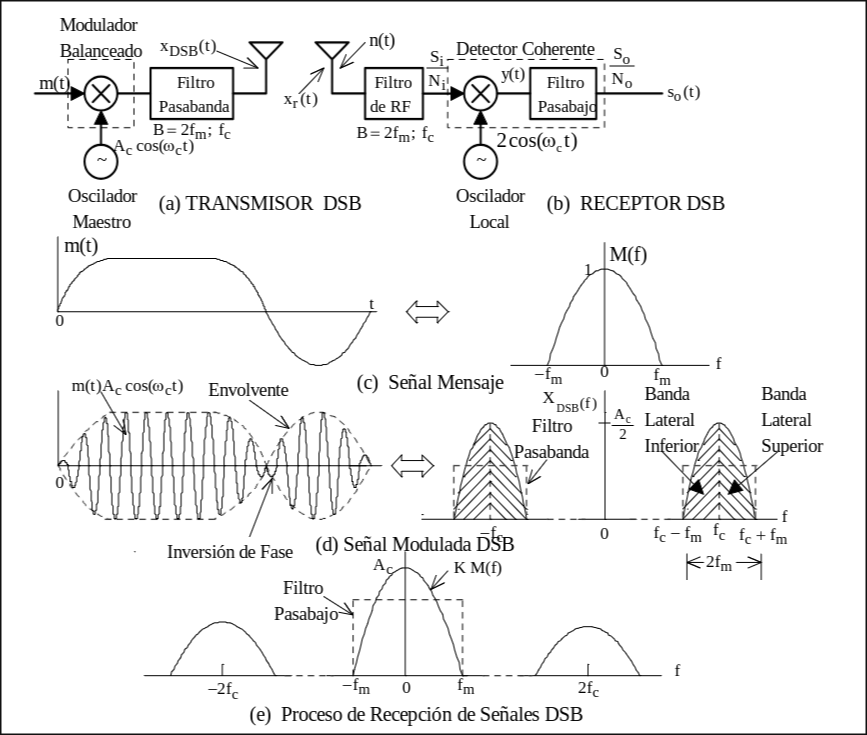
\includegraphics[width=0.9\textwidth]{modulacion_dsb.png}
  \caption{Modulación de Amplitud de Doble Banda Lateral con Portadora Suprimida}
  \label{fig:Modulacion DSB}
\end{figure}
Es eficiente ya que toda la potencia va a las bandas, pero tiene algunas serias desventajas: La envolvente de $x_{DSB}(t)$ es $\lvert m(t) \rvert$, no $m(t)$ por lo que precisa detección coherente (que es más compleja y cara), es un sistema de banda angosta y la más grave de todas, requiere perfecta sincronización de la portadora local, ya que si hay errores de frecuencia $\Delta f$ o de fase $\Delta \phi$ puede resultar en atenuación, desvanecimiento, inversión de la señal o incluso puede desaparecer si el oscilador está desfasado en $\Delta \phi = \pi$.  

\subsubsection{Modulación de Amplitud con Portadora de gran Potencia (AM)}
Para subsanar la limitación basica de sincronización de la modulación DSB, el método de “Modulación AM” se obtiene con una simple adición al sistema DSB ya visto: transmitir la portadora junto con la señal, evitando de esta forma la necesidad de generar una copia exacta de la portadora en el receptor. De esta forma, tenemos que $m_c(t)=0$, $A(t)=m_c(t)=[A_c+m(t)]$ y $\phi = 0$ por lo que resulta:
\begin{equation}
  x_{AM}(t)=[A_c + m(t)]\cos(2\pi f_ct)=m(t)\cos(2\pi f_ct) + A_c\cos(2\pi f_ct)
\end{equation}
Donde $A(t)=[A_c+m(t)]$ es la amplitud de la portadora modulada. Suponemos también que $\langle m(t)\rangle =0$. El primer término de $x_{AM}(t)$ es una señal DSB y el segundo término la portadora agregada. Por lo tanto, el espectro correspondiente será:
\begin{equation}
  X_{AM}(f)=\frac{A_c}{2}[\delta (f+f_c) + \delta (f-f_c)] + \frac{1}{2} [M(f+f_c) + M(f-f_c)]
\end{equation}
El sistema de modulación AM primero en el receptor adiciona $A_c$ al mensaje $m(t)$ y luego multiplica por la portadora sinusoidal (modulador AM), y tras pasarlo por un filtro pasabanda, la modulada sale por la antena. Luego, el receptor recibe la señal atenuada y con ruido, la pasa por un filtro de RF y utiliza un detector de envolvente para quedarse con $E(t)$, la cual filtra con un filtro de pasabajos para demodular la señal.
\begin{figure}[H]
  \centering
  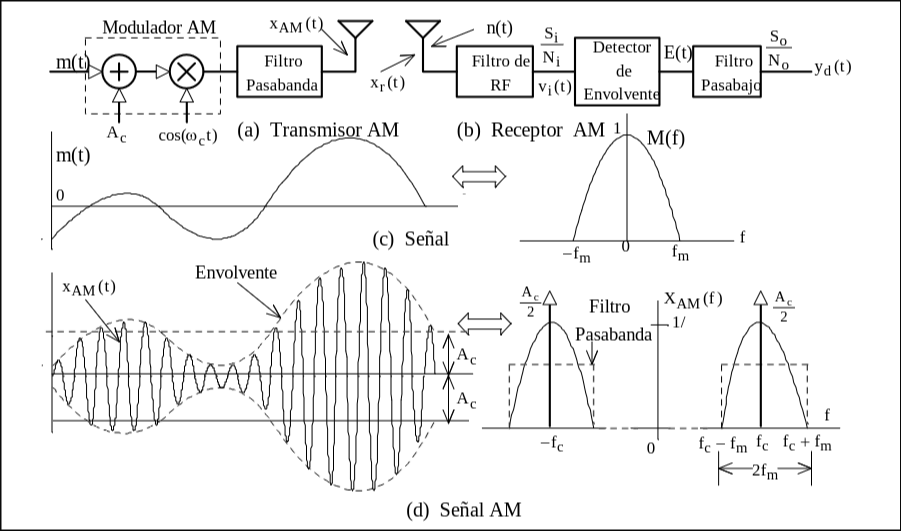
\includegraphics[width=0.9\textwidth]{modulacion_am.png}
  \caption{Modulación de Amplitud}
  \label{fig:Modulacion AM}
\end{figure}
La envolvente de la señal modulada es la señal mensaje desplazada en una constante $A_c$. Esta propiedad permite la extracción de la información mediante un detector de envolvente mientras la constante $A_c$ sea lo suficientemente alta para preservar la forma de la envolvente. Si no se cumple con esto, la envolvente pierde su forma y resulta muy difícil o imposible recuperar $m(t)$, en lo que se conoce como “sobremodulación”. Para evitar la sobremodulación, establecemos ciertas condiciones para $A_c$ y algunos parámetros de interés:

Suponiendo que $\langle m(t)\rangle =0$, el mensaje $m(t)$ se puede escribir de la forma siguiente: $m(t)= \lvert \min m(t) \rvert m_n(t)$ donde $\lvert \min m(t) \rvert$ es la máxima excursión negativa de $m(t)$ mientras que $m_n(t)$ es el mensaje normalizado tal que $\lvert \min m(t) \rvert = 1$. Reemplazando en la expresión que tenemos de modulada resulta:
\begin{equation}
  \begin{aligned}
    x_{AM}(t)&=[A_c + \lvert \min m(t) \rvert m_n(t)]\cos(2\pi f_ct)\\
    x_{AM}(t)&=A_c[1 + a\,m_n(t)]\cos(2\pi f_ct),\quad a=\frac{\lvert \min m(t) \rvert}{A_c}
  \end{aligned}
\end{equation}
El término $a$ se define como “índice de modulación AM”. Es evidente que la envolvente $A(t) = A_c[1 + a\,m_n(t)]$ debe ser siempre positiva y, por inspección del gráfico (d) de la Figura~\ref{fig:Modulacion AM} solo se cumple cuando $A_c \geq \lvert \min m(t) \rvert$, lo cual implica que $0<a<1$. La detección de envolvente se podrá emplear siempre que el índice de modulación $a$ sea igual o menor que la unidad; en estas condiciones la envolvente de la señal AM jamás cruzará el eje $t$ y la porción positiva de la envolvente será una réplica desplazada del mensaje.

Como en general la salida del detector de envolvente se aplica a un filtro pasabajo, la componente continua es eliminada, pero también son eliminadas muchas componentes de baja frecuencia de la señal mensaje. Por consiguiente, el sistema AM no es el más apropiado para la transmisión de señales con fuertes componentes de baja frecuencia.

\subsubsection{Potencia y Rendimiento de Transmisión en AM}
La potencia total $P_T$ de la señal modulada AM es de:
\begin{equation}
  P_T=\langle x_{AM}^2(t)\rangle =\frac{1}{2}\langle A_c^2 + 2A_cm(t) + m^2(t)\rangle 
\end{equation}
Pero como $\langle m(t)\rangle  = 0$, entonces:
\begin{equation}\label{eq:PT_AM}
  P_T=\langle x_{AM}^2(t)\rangle =\frac{1}{2}<A_c^2 +\frac{1}{2}\langle m^2(t)\rangle =P_c+P_B
\end{equation}
El primer término de \eqref{eq:PT_AM} $P_c$ es la potencia de la portadora, mientras que el segundo $P_B$ es la potencia útil que contiene información y está contenida en las bandas laterales.

Luego, podemos definir el rendimiento de transmisión $E\%$ como:
\begin{equation}\label{eq:E_AM}
  E\%=\frac{P_B}{P_B+P_c}100=\frac{\langle m^2(t)\rangle }{A_c^2+\langle m^2(t)\rangle }100
\end{equation}
Y puesto que $m(t)=a\,A_cm_n(t)$ también podemos expresar $E\%$ como:
\begin{equation}
  E\%=\frac{a^2\langle m_n^2(t)\rangle }{1+a^2\langle m_n^2(t)\rangle }100
\end{equation}
Como vimos previamente, la detección de envolvente solo se puede usar cuando $a\leq1$, y como $\langle m_n^2(t)\rangle \leq1$, se verifica que el rendimiento máximo en AM es del 50\% y se obtiene cuando $m(t)$ es una señal periódica bipolar de amplitud $\pm1$. En el caso de DSB, al no tener portadora, toda la potencia transmitida es útil y por lo tanto su rendimiento es del 100\%.
\subsubsection{Ancho de Banda y Relaciones S/N en AM}
La modulación AM es también una modulación de doble banda lateral y por lo tanto su ancho de banda es $B=2f_m$ donde $f_m$ es la frecuencia máxima de la señal mensaje $m(t)$.

La relación de expansión del ancho de banda $\beta_m=\frac{B}{f_m}$ es igual a 2, por lo que el sistema de modulación AM es de banda angosta en el cuál no hay posibilidad de intercambio “Ancho de Banda-Relación S/N”

En tanto al efecto del ruido en la modulación AM:

La señal recibida se puede expresar como:
\begin{equation}
  x_r(t)=[A_r + m(t)]\cos(2\pi f_ct)=A_r\cos(2\pi f_ct)+m(t)\cos(2\pi f_ct)
\end{equation}
Esta señal aparece a la entrada de nuestro detector de envolventes con potencia:
\begin{equation}
  S_i=\langle x_r^2(t)\rangle =\frac{1}{2}A_r+\frac{1}{2}\langle m^2(t)\rangle 
\end{equation}
El ruido a la entrada del detector es ruido blanco pasabanda de densidad espectral $\frac{\eta}{2}$ y se puede representar como:
\begin{equation}
  n(t)=n_c(t)\cos(2\pi f_ct)+n_s(t)\sin(2\pi f_ct)=R_n(t)\cos(2\pi f_ct)
\end{equation}
Y su potencia a la entrada del detector resulta:
\begin{equation}
  N_i=\langle n^2(t)\rangle =\langle n_c^2(t)\rangle =\langle n_s^2(t)\rangle =2\eta f_m
\end{equation}
Y la relación Signal to Noise de entrada será de:
\begin{equation}
  \frac{S_i}{N_i}=\frac{A_r^2+\langle m^2(t)\rangle }{2N_i}
\end{equation}
A la salida del detector tendremos dos casos según si la potencia de la señal es mucho mayor o mucho menor que la de ruido. Si es mucho menor, la señal queda “capturada” en el ruido o inmersa en ruido multiplicativo y no tiene sentido hablar de S/N ya que la inteligibilidad será nula. Sin embargo, si es mucho mayor, tenemos que $S_o=\langle m^2(t)\rangle $ y $N_o=\langle n_c^2(t)\rangle =N_i$ y por ende:
\begin{equation}
  \frac{S_o}{N_o}=\frac{\langle m^2(t)\rangle }{N_i}
\end{equation}
La ganancia de conversión de AM será:
\begin{equation}
  \frac{S_o/N_o}{S_i/N_i} = 2\frac{\langle m^2\rangle }{A_r^2}
\end{equation}
Pero por la ecuación \eqref{eq:E_AM} sabemos que la expresión a la derecha del igual es lo mismo que el doble del rendimiento de transmisión, cuyo valor máximo es 50\%, luego la ganancia de conversión cumple que:
\begin{equation}
  \frac{S_o/N_o}{S_i/N_i}\leq1,\quad \left[\frac{S_o/N_o}{S_i/N_i}\right]_{max}=1
\end{equation}

\subsection{Modulación en Ángulo}
Las señales moduladas en ángulo son señales de envolvente constante y la información esta contenida en la fase instantánea de la portadora. Si tomamos $A(t)=A_c$ constante, resulta en la expresión:
\begin{equation}\label{eq:x_ang}
  x_c(t)=A_c\cos[\theta(t)]=A_c\cos[2\pi f_ct + \phi(t)]
\end{equation}
Donde $\theta(t)=[2\pi f_ct + \phi(t)]$ es el ángulo o fase instantánea de la portadora y $\phi(t)$ es la desviación instantánea de fase. Además, definimos frecuencia instantánea $f_i(t)$ como:
\begin{equation}
  f_i(t)=\frac{1}{2\pi}\frac{d}{dt}[\theta(t)]=f_c+\frac{1}{2\pi}\frac{d}{dt}\phi(t)
\end{equation}
También definimos:
\begin{equation}
  \begin{aligned}
    &\Delta\phi=\lvert\phi(t)\rvert_{max} = \text{ desviación máxima de fase}\\
    &\Delta f(t)=\frac{1}{2\pi}\frac{d}{dt}\phi(t) = \text{ desviación instantánea de frecuencia}\\
    &\Delta f=\lvert\Delta f(t)\rvert_{max}= \text{ desviación máxima de frecuencia}
  \end{aligned}
\end{equation}
La desviación instantánea de fase $\phi(t)$ está relacionada con la señal mensaje y dependiendo de la naturaleza de esa relación se tienen los tipos de modulación en ańgulo.

\subsubsection{PM}
La modulación de fase (Phase Modulation) es aquella en la que la desviación de fase instantánea $\phi (t)$ es proporcional a la señal mensaje, es decir:
\begin{equation}
  \phi(t)=k_pm(t)
\end{equation}
Donde $k_p$ es la constante de desviación de fase del modulador y se expresa en radianes por unidad de $m(t)$.

La modulada en PM resulta:
\begin{equation}
  x_{PM}(t)=A_c\cos[2\pi f_c t + k_pm(t)]
\end{equation}
Además, definimos el índice de modulación angular $\beta$ en la forma:
\begin{equation}
  \beta_p = k_pA_m
\end{equation}

\subsubsection{FM}
La modulación de frecuencia (Frecuency Modulation) es aquella en la que la desviación instantánea de frecuencia $\Delta f(t)$ es proporcional a la señal mensaje $m(t)$, es decir:
\begin{equation}\label{eq:df_FM}
  \Delta f(t)=\frac{1}{2\pi}\frac{d}{dt}\phi (t)=f_dm(t)
\end{equation}
O también mediante integración de \eqref{eq:df_FM}, obtenemos que la desviación instantánea de fase es proporcional a la integral de la señal mensaje:
\begin{equation}
  \phi (t)=2\pi f_d\int_{t_0}^{t} m(\tau) \,d\tau + \phi_0(t_0)
\end{equation}
La constante $f_d$ es la constante de desviación de frecuencia del modulador. Algunas veces se define $k_f=2\pi f_d$. El valor de la constante $\phi_0(t_0)$ es la desviación de fase $t=t_0$ que podemos hacerla igual a 0 sin perder generalidad (según el libro).

La modulada en FM resulta:
\begin{equation}
  x_{FM}(t)=A_c\cos[2\pi f_c t + 2\pi f_d\int_{}^{t} m(\tau) \, d\tau]
\end{equation}
Además, definimos el índice de modulación angular $\beta$ en la forma:
\begin{equation}
  \beta = \frac{f_dA_m}{f_m}=\frac{\Delta f}{f_m}=\Delta \phi
\end{equation}
Usamos FM cuando importa la alta fidelidad y el ancho de banda no es limitante, como en radiodifusión FM, audio de TV, microondas y comunicaciones móviles punto a punto.

\subsubsection{Generación de señales FM}
Como la señal FM tiene envolvente constante, diseñar generadores y detectores resulta más fácil. No hay picos que provoquen disipación excesiva en los dispositivos. Además, el ruido aditivo casi no afecta a la información, porque esta va en los cruces por cero. En cambio, las variaciones espurias de frecuencia sí hacen daño, porque el detector las interpreta como variaciones de amplitud. Para generar señales FM, hay dos familias: generadores directos y generadores indirectos.

En la generación directa, la frecuencia de la portadora se modula directamente con la señal. Alcanza con un oscilador controlado por tensión (VCO), cuya frecuencia de oscilación depende de la tensión de entrada. Como la frecuencia de la portadora tiende a ser inestable, se suele usar un VCO seguido de multiplicadores de frecuencia y un mezclador, con un oscilador que estabiliza la portadora.

\begin{figure}[H]
  \centering
  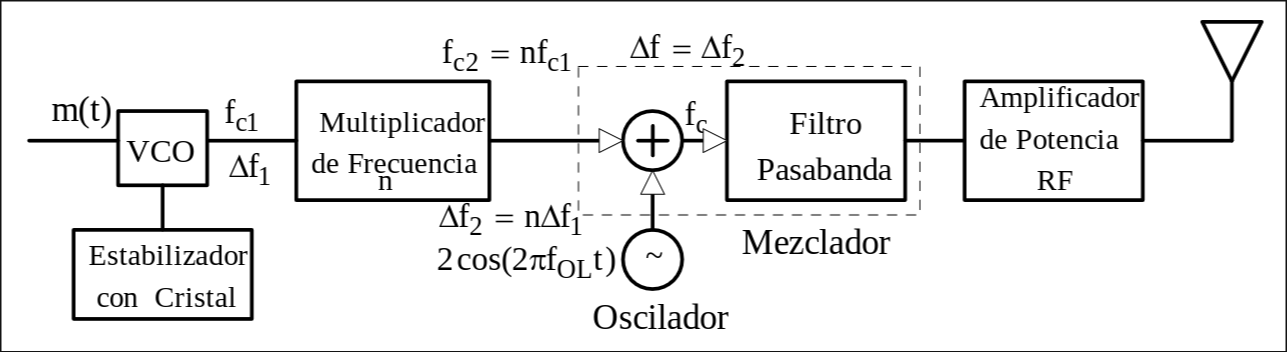
\includegraphics[width=0.9\textwidth]{fm_directa.png}
  \caption{Transmisor FM con VCO y Multiplicación de Frecuencia}
  \label{fig:FM Directa}
\end{figure}

En la generación indirecta, no se modula la frecuencia directamente. Primero se genera una señal de banda angosta con un modulador de fase, que usa una portadora de cristal muy estable, y después se la lleva a banda ancha con multiplicadores de frecuencia. El proceso sigue este orden. La señal $m(t)$ pasa por un integrador, de modo que la modulación de fase posterior se comporta como FM. Luego entra al modulador de fase de banda angosta, que produce una señal FM con desviación muy pequeña. Después va a un primer multiplicador $(n_1)$, que aumenta la portadora y la desviación. El mezclador traslada el espectro sin cambiar su ancho de banda, y un segundo multiplicador $(n_2)$ vuelve a multiplicar. Por último, el amplificador de potencia de RF entrega la señal. Los factores de multiplicación los fija la desviación máxima que se quiere lograr. Como el resultado puede no coincidir con la portadora de transmisión $f_c$, el mezclador traslada el espectro a la frecuencia correcta. Se coloca en el medio de la cadena para que las frecuencias intermedias no resulten demasiado altas.

\begin{figure}[H]
  \centering
  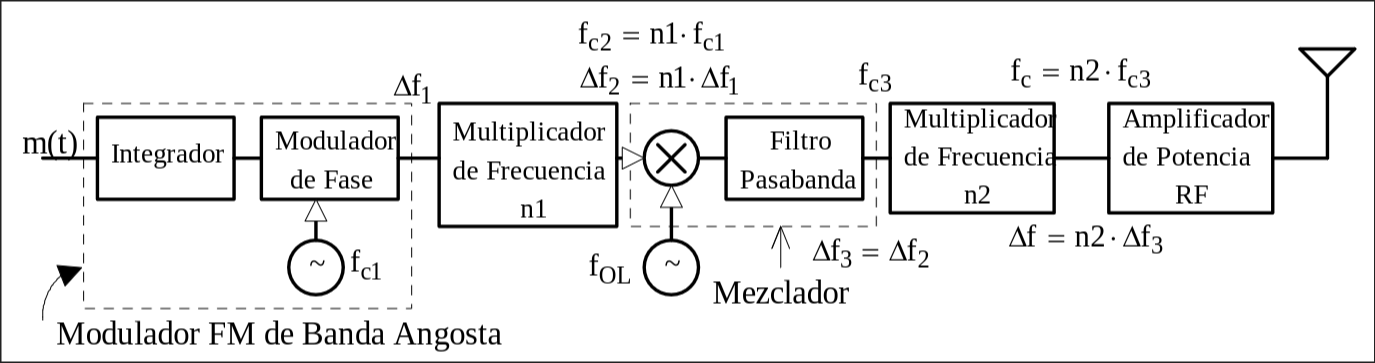
\includegraphics[width=0.9\textwidth]{fm_indirecta.png}
  \caption{Transmisor Armstrong de FM Indirecta}
  \label{fig:FM Indirecta}
\end{figure}

\subsubsection{Detección de señales FM}
La demodulación de una señal modulada FM requiere un dispositivo cuya salida sea proporcional a la frecuencia de entrada. Estos dispositivos se denominan comúnmente “discriminadores”. Si la entrada al discriminador es una señal modulada en ángulo de la forma $x_r(t)=A_r\cos[2\pi f_ct + \phi(t)]$, la salida del discriminador ideal es:
\begin{equation}
  y_D(t)=\frac{k_D}{2\pi}\frac{d}{dt}\phi(t)
\end{equation}
Pero en FM $\phi(t)=2\pi f_d\int_{}^{t} m(\tau) \, d\tau$ y $\frac{d}{dt}\phi(t)=2\pi f_d m(t)$, entonces:
\begin{equation}
  y_D(t)=k_Df_dm(t)=k_D\Delta f(t)
\end{equation}

\begin{figure}[H]
  \centering
  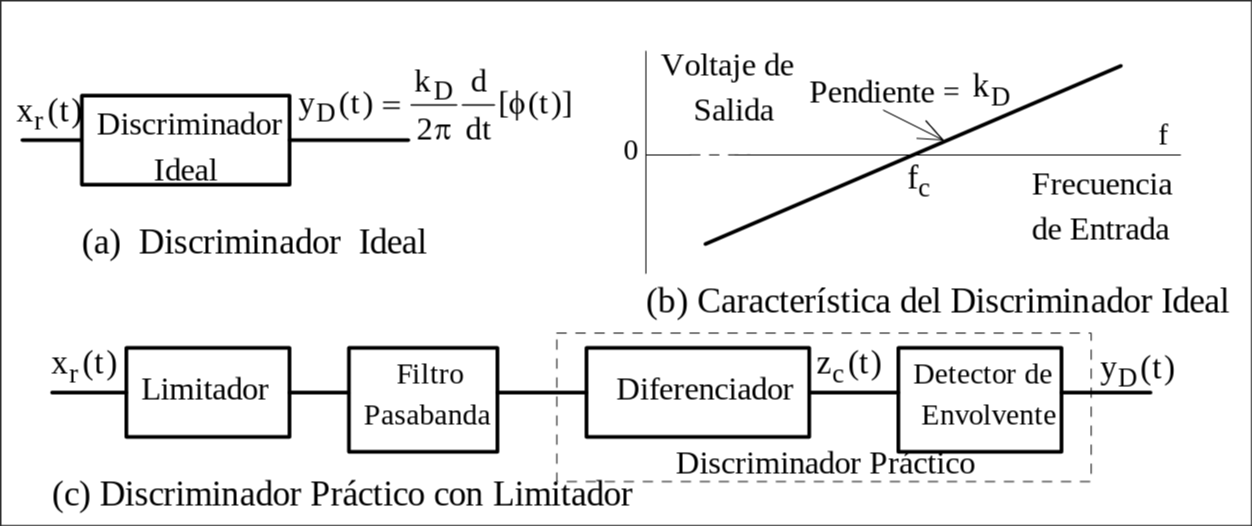
\includegraphics[width=0.9\textwidth]{fm_discriminador.png}
  \caption{Discriminador de Señales Moduladas en Frecuencia}
  \label{fig:FM Discriminador}
\end{figure}
El discriminador se puede instrumentar en la práctica mediante un diferenciador seguido de un detector de envolvente, como se muestra en la Figura~\ref{fig:FM Discriminador}. El diferenciador convierte la FM en una señal tipo AM cuya envolvente es $E(t)=A_r[f_c + f_dm(t)]$, y el detector la recupera sin distorsión si $f_c \geq \Delta f$.

Esta forma de demodulación de señales FM se denomina “demodulación por detección de pendiente”. Uno de los principales problemas con este método es que el detector es muy sensible a variaciones espurias en la amplitud de la señal FM debidas al ruido aditivo. A fin de asegurarse que la amplitud de la entrada al diferenciador sea constante, se coloca a su entrada un limitador. Este limitador recorta la señal de entrada y la convierte en una señal cuasi-rectangular que lleva la información en los cruces por cero. Esta señal se filtra en un filtro pasabanda centrado en $f_c$ para convertirla en la forma cuasi-sinusoidal requerida por el detector de envolvente. Normalmente el limitador y el filtro pasabanda están integrados en la misma unidad, conocida como “limitador pasabanda”.

\begin{figure}[H]
  \centering
  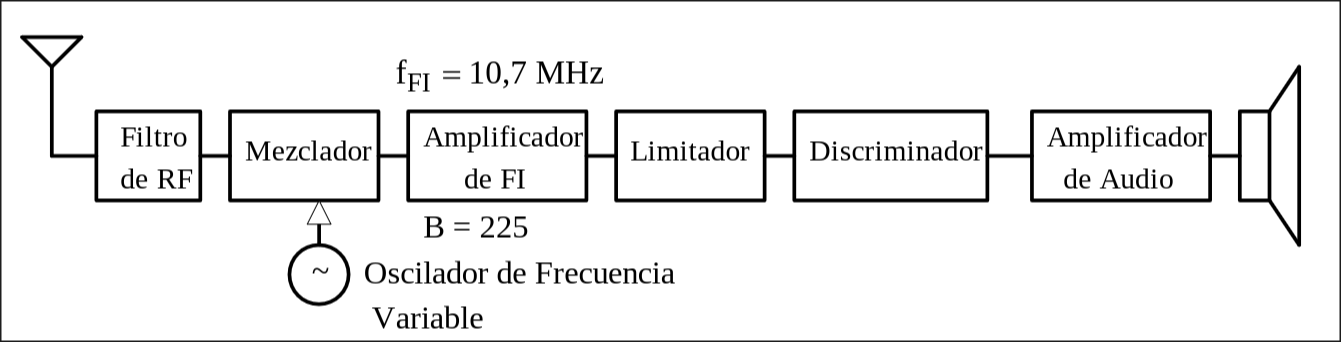
\includegraphics[width=0.9\textwidth]{fm_receptor.png}
  \caption{Diagrama de Bloques de un Receptor FM típico}
  \label{fig:FM Receptor}
\end{figure}

\subsubsection{Banda Angosta}
Partiendo de la ecuación \eqref{eq:x_ang}, si $\phi (t)$ es muy chico, los valores del índice de modulación $\beta < \frac{\pi}{2}$ y por ende $\cos\phi \approx 1$ y $\sin\phi \approx \phi$. Luego, resulta en:
\begin{equation}
  \begin{aligned}
    &x_c(t) \approx A_c\cos(2\pi f_ct) - A_c\phi (t)\sin(2\pi f_c t)\\
    &X_c(f) = \frac{A_c}{2}[\delta (f+f_c) + \delta (f-f_c)] + \frac{A_c}{2j}[\Phi (f+f_c) - \Phi (f-f_c)]
  \end{aligned}
\end{equation}
Donde el primer término es la portadora y el segundo es la misma portadora multiplicada por $\phi (t)$ en cuadratura $(90^\circ)$, y genera las bandas laterales. Por lo tanto, si $\phi (t)$ tiene ancho de banda $B$, entonces $B_T= 2B$, al igual que en AM solo que en AM las bandas laterales están en fase mientras que acá están desfasadas $\frac{\pi}{2}$.

\subsubsection{Banda Ancha}
Para valores grandes de $\phi (t)$, $\beta > \frac{\pi}{2}$ por lo tanto no podemos simplificar el seno y el coseno y hay que quedarse con la función $\phi (t)$ completa, lo que genera más componentes de frecuencia. La fase de la portadora oscila $\beta$ radianes ida y vuelta $f_m$ veces por segundo, resultado de mezclar la portadora con armónicos de $f_m$. Matemáticamente, eso es el desarrollo en funciones de Bessel:
\begin{equation}
  x_c(t) = A_c\sum_{n=-\infty}^{\infty} J_n(\beta)\cos[2\pi(f_c+nf_mt)]
\end{equation}
Cada término es una línea espectral en $f_c+n\,f_m$ con amplitud $A_cJ_n(\beta)$, de modo tal que en $n=0$ está la portadora con amplitud $A_cJ_0(\beta)$ y todas las demás son bandas laterales. Además, $J_n(\beta)$ es despreciable cuando $n>\beta$, por lo que de ahí sacamos las bandas laterales que nos importan.

Luego, partiendo de $\beta = \frac{\Delta f}{f_m}$ el ancho de banda en FM de banda ancha se calcula como $B_T=2(\beta+1)f_m$. 

\subsubsection{Potencia y Rendimiento en FM}
Como la envolvente de la señal es constante en modulación angular, la potencia promedio tanto en banda angosta como en banda ancha es:
\begin{equation}
  P_T=\langle x_c^2(t)\rangle =\frac{A_c}{2}\left[ J_0^2(\beta) + 2 \sum_{n=1}^{\infty} J_n^2(\beta) \right]=\frac{A_c^2}{2}
\end{equation}
En este caso, la potencia total no cambia con el índice de modulación, sino que varía cuanta potencia va en la portadora y cuanta va en las bandas laterales.

Luego, si un filtro deja pasar solamente k laterales a cada lado, definimos fracción de potencia transmitida como:
\begin{equation}
  P_r=J_0^2(\beta) + 2 \sum_{n=1}^{k} J_n^2(\beta)
\end{equation}
Con $P_r \geq 0,98$ se cumple que $k \approx \lfloor \beta + 1 \rfloor$, y de $B_T=2kf_m$ resulta $B_T\approx 2(\beta + 1)f_m$, que contiene siempre (usando la tabla de Bessel) el $98\%$ de la señal.

\subsubsection{Relacion S/N en FM}
A partir del esquema del receptor, asumiendo que podemos separar el ruido y la señal para calcularlos (es decir, $m(t)=0$ para calcular el ruido y que no hay ruido para la señal) tenemos:
\begin{equation}
  \frac{S_i}{N_i}=\frac{A_r^2}{2\eta B_T} \qquad \text{(predetección)}
\end{equation}
\begin{equation}
  \frac{S_o}{N_o}=\frac{3A_r^2f_d^2\langle m^2(t)\rangle }{2\eta f_m^3} \qquad \text{(postdetección)}
\end{equation}
El ruido a la salida del discriminador no es plano, es parabólico (crece con $f^2$) y por eso $N_o=\frac{2}{3} \left( \frac{k_D}{A_r} \right)^2\eta f_m^3$.

Luego, la ganancia de conversión resulta:
\begin{equation}
  \frac{S_o/N_o}{S_i/N_i}=\frac{3}{4} \left( \frac{B_T}{f_m} \right)^3 \langle m^2(t)\rangle .
\end{equation}

\subsection{¿Múltiples Canales?}
La FDM es una operaci\'on mediante la cual varias se\~nales diferentes se transmiten conjunta y simult\'aneamente por un mismo canal, utilizando subportadoras y traslaci\'on de frecuencias. El espectro de cada se\~nal se traslada a una banda diferente, y el espectro compuesto forma una banda base que puede transmitirse con cualquiera de los esquemas de modulaci\'on vistos.

\subsubsection{Transmisor}
Cada se\~nal individual modula una subportadora diferente $f_{c_i}$ (generalmente de baja frecuencia). Las se\~nales moduladas se suman en un combinador, y la se\~nal compuesta, la banda base, modula un transmisor de RF.

\subsubsection{Receptor}
El receptor de RF, cuyo ancho de banda debe alcanzar para la se\~nal multicanal, demodula la se\~nal compuesta y la aplica a una bater\'ia de filtros pasabanda centrados en las subportadoras. Cada ancho de banda debe dise\~narse para dejar pasar solo el espectro de su se\~nal. Luego cada mensaje se detecta seg\'un el tipo de modulaci\'on empleado en el transmisor.

\subsubsection{Banda de Guarda y Ancho de Banda}
Para que no haya solapamiento entre espectros se agrega una banda de guarda $B_g$, que tambi\'en facilita la recuperaci\'on de cada se\~nal con filtros pr\'acticos. El ancho de banda de la banda base de $M$ se\~nales multiplexadas es
\begin{equation}
  B_T = (M-1)B_g + \sum_{m=1}^{M} B_m
\end{equation}
donde $B_1, B_2, \dots, B_M$ son los anchos de banda de las se\~nales individuales, que dependen del tipo de modulaci\'on, que en nuestro caso es:
\begin{equation}
  B = 2f_m \;\; (\text{AM o DSB})
\end{equation}

Luego, vemos lo detallado en la siguiente figura:

\begin{figure}[H]
  \centering
  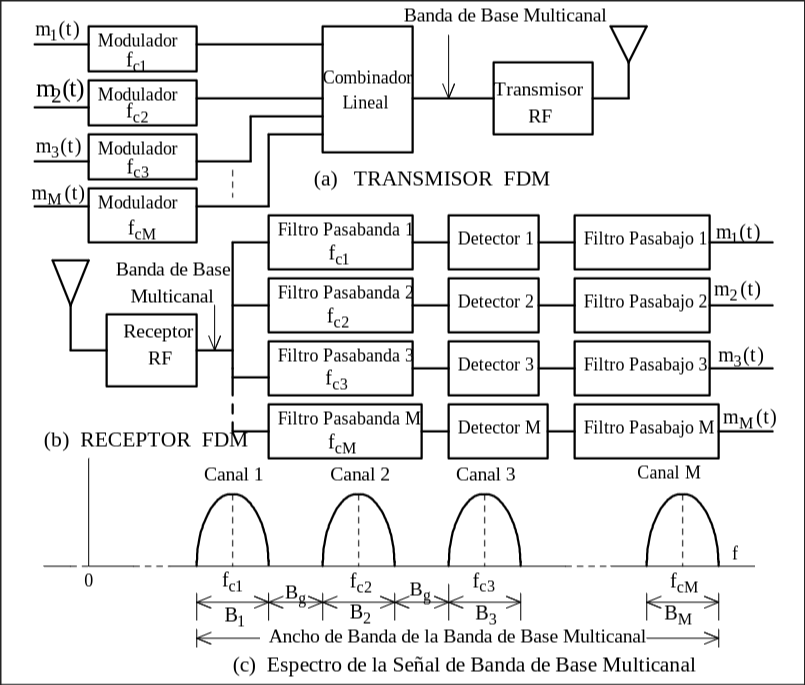
\includegraphics[width=0.9\textwidth]{fdm.png}
  \caption{Multiplicidad por División de Frecuencias (FDM)}
  \label{fig:FDM}
\end{figure}

\section{Implementación}

\subsection{Herramientas}
La simulación se implementó en Python con \texttt{numpy} (generación de señales y FFT), \texttt{scipy} (funciones de Bessel, envolvente y densidad espectral de potencia), \texttt{matplotlib} (gráficos) y \texttt{soundfile} (lectura y escritura de audio). El código está en \texttt{codigo/modulacion.py} y el cuaderno \texttt{codigo/proyecto2.ipynb} permite ver todas las figuras y escuchar las señales (ver Anexo).

\subsubsection{La Transformada Rápida de Fourier (FFT)}
La transformada de Fourier $X(f)=\int_{-\infty}^{\infty}x(t)\,e^{-j2\pi ft}\,dt$ sólo puede resolverse analíticamente para señales sencillas, y una computadora únicamente maneja una cantidad finita de valores de la señal. Por eso los espectros se calculan con la Transformada de Fourier Discreta (DFT), que reemplaza la integral por una suma, y la FFT es el algoritmo que calcula la DFT en forma eficiente (Briceño, Apéndice A). En el proyecto se usa para obtener los espectros y para aplicar los filtros, el derivador y el integrador del receptor en el dominio de la frecuencia.

\subsection{Parámetros de Diseño}
\paragraph{Número de señales.} El sistema transmite $M=2$ canales multiplexados en frecuencia:
\begin{itemize}
  \item Canal 1: tono de prueba $m_1(t)=50\cos(2\pi\,440\,t)$ V (nota La4).
  \item Canal 2: $5$ s de \textit{La Marcha Imperial} (\texttt{assets/imperial\_march.wav}).
\end{itemize}

\paragraph{Parámetros comunes.} En todos los esquemas la portadora tiene $A_c=100$ V, por lo que la potencia de la portadora sin modular es $P_c=A_c^2/2=5000$ W (sobre 1 $\Omega$). El canal agrega ruido blanco de densidad espectral $\eta/2$, con $\eta=10^{-3}$ W/Hz. Cada canal ocupa su propia subportadora:

\begin{table}[H]
  \centering
  \begin{tabular}{lcccc}
    \toprule
    Esquema & $f_{c1}$ (tono) & $B_1$ & $f_{c2}$ (audio) & $B_2$ \\
    \midrule
    AM            & 20 kHz & 880 Hz   & 50 kHz & 10 kHz \\
    FM banda angosta & 20 kHz & 1,06 kHz & 80 kHz & 12 kHz \\
    FM banda ancha   & 20 kHz & 5,28 kHz & 80 kHz & 60 kHz \\
    PM               & 20 kHz & 5,28 kHz & 80 kHz & 24,4 kHz \\
    \bottomrule
  \end{tabular}
  \caption{Plan de subportadoras FDM y ancho de banda de cada canal.}
  \label{tab:plan}
\end{table}

\paragraph{Receptor.} Cada canal se separa con un filtro pasabanda ideal de ancho $B_i$ centrado en su subportadora y luego se demodula:
\begin{itemize}
  \item AM: detector de envolvente ideal, filtro pasabajo de ancho $f_m$ y bloqueo de la continua $A_c$ (el capacitor de salida).
  \item FM: discriminador de la Figura \ref{fig:FM Receptor}, formado por un limitador pasabanda ideal (deja $\cos\theta(t)$ con amplitud constante), un diferenciador ideal $H(f)=j2\pi f$ y un detector de envolvente. A la salida se obtiene $E(t)=2\pi[f_c+f_dm(t)]$; restando $f_c$ y dividiendo por $f_d$ queda $m(t)$.
  \item PM: el mismo discriminador seguido de un integrador de ganancia $2\pi$ y dividido por $k_p$, como indica Briceño para la recepción de PM.
\end{itemize}

\subsection{Canal 1: Tono Puro}
Usando $m(t)=50\cos(2\pi 440t)$ que corresponde a la nota musical La(A) en la octava 4, de potencia $\langle m^2(t)\rangle =\frac{A_m^2}{2}=\frac{(50\,\mathrm{V})^2}{2}=1250\,\mathrm{V}^2$:
\subsubsection{Modular en Amplitud (AM)}
Tomo una portadora de amplitud $A_c=100\,\mathrm{V}$ y frecuencia $f_c=20\,\mathrm{kHz}$ y modulo el tono:
\begin{equation}
  x_{AM}(t)=[100\,\mathrm{V} + 50\,\mathrm{V}\cos(2\pi 440\,\mathrm{Hz}\,t)]\cos[2\pi (20 \times 10^3)\,\mathrm{Hz}\,t]
\end{equation}
De la cual podemos calcular:

\textbf{Índice de Modulación:}
\begin{equation}
  a = \frac{\lvert \min m(t) \rvert}{A_c}=\frac{50\,\mathrm{V}}{100\,\mathrm{V}}=0,5
\end{equation}
\textbf{Potencia Total:}
\begin{equation}
  P_T=\langle x_{AM}^2(t)\rangle =\frac{A_c^2}{2} + \frac{\langle m^2(t)\rangle }{2}= P_c + P_B = 5000\,\mathrm{W} + 625\,\mathrm{W} = 5625\,\mathrm{W}
\end{equation}
\textbf{Rendimiento de Transmisión:}
\begin{equation}
  \begin{aligned}
    E\%&=\frac{P_B}{P_B+P_c}\times 100=\frac{625\,\mathrm{W}}{5625\,\mathrm{W}}\times 100\\
       &=\frac{a^2\langle m_n^2(t)\rangle }{1+a^2\langle m_n^2(t)\rangle }\times 100=\frac{0,25\cdot 0,5}{1+0,25\cdot 0,5}\times 100\approx 11,11\%
  \end{aligned}
\end{equation}
\textbf{Ancho de Banda:}
\begin{equation}
  B_T=2f_m=2\times440\,\mathrm{Hz}=880\,\mathrm{Hz}
\end{equation}
Por ser modulación sinusoidal, el espectro tiene sólo tres líneas: la portadora en $f_c$ con amplitud $A_c/2=50$ V y las bandas laterales en $f_c\pm 440$ Hz con amplitud $A_m/4=12,5$ V (espectro bilateral, Briceño Fig. 6.6).

\subsubsection{Modular en Ángulo (FM y PM)}
Tomo una portadora de amplitud $A_c=100\,\mathrm{V}$ y frecuencia $f_c=20\,\mathrm{kHz}$ y modulo el tono:
\begin{equation}
  x_{FM}(t)=100\,\mathrm{V}\cos\left[ 2\pi (20\times 10^3)\,\mathrm{Hz}\,t + 2\pi f_d\int_{}^{t} 50\,\mathrm{V}\cos(2\pi 440\,\mathrm{Hz}\,\tau)\, d\tau \right]
\end{equation}
\begin{equation}
  x_{PM}(t)=100\,\mathrm{V}\cos[2\pi (20\times 10^3)\,\mathrm{Hz}\,t + k_p\,50\,\mathrm{V}\cos(2\pi 440\,\mathrm{Hz}\,t)]
\end{equation}
La envolvente es constante, así que la potencia total es siempre $P_T=\frac{A_c^2}{2}=5000\,\mathrm{W}$. El índice $\beta$ determina cómo se reparte esa potencia: la portadora queda con $P_c=\frac{A_c^2}{2}J_0^2(\beta)$ y el resto, $\frac{A_c^2}{2}[1-J_0^2(\beta)]$, va a las bandas laterales.

Para FM de banda angosta se debe cumplir que $\beta < \frac{\pi}{2}$, y como $\beta =\frac{f_dA_m}{f_m}=f_d\frac{50\,\mathrm{V}}{440\,\mathrm{Hz}}$ despejamos $f_d$ para $\beta = 0,2$ en banda angosta y $\beta = 5$ en banda ancha:

\textbf{Banda angosta} ($\beta=0,2 \Rightarrow f_d=\frac{0,2\cdot 440\,\mathrm{Hz}}{50\,\mathrm{V}}=1,76$ Hz/V, $\Delta f=\beta f_m=88$ Hz):
\begin{equation}
  x_{FM}(t)=100\,\mathrm{V}\cos\left[ 2\pi (20\times 10^3)\,\mathrm{Hz}\,t + 2\pi\, 1,76\,\mathrm{Hz/V}\int_{}^{t} 50\,\mathrm{V}\cos(2\pi 440\,\mathrm{Hz}\,\tau)\, d\tau \right]
\end{equation}
\begin{equation}
  \begin{aligned}
    &P_c=5000\,\mathrm{W}\cdot J_0^2(0,2)=4900,7\,\mathrm{W}\;(98\%),\qquad P_B=99,3\,\mathrm{W}\\
    &B_T=2(\beta+1)f_m=1056\,\mathrm{Hz}\approx 2f_m
  \end{aligned}
\end{equation}
Las bandas laterales en $f_c\pm f_m$ tienen amplitud $A_c\beta/4=5$ V, como en AM, pero con la lateral inferior de signo contrario.

\textbf{Banda ancha} ($\beta=5 \Rightarrow f_d=\frac{5\cdot 440\,\mathrm{Hz}}{50\,\mathrm{V}}=44$ Hz/V, $\Delta f=2200$ Hz):
\begin{equation}
  x_{FM}(t)=100\,\mathrm{V}\cos\left[ 2\pi (20\times 10^3)\,\mathrm{Hz}\,t + 2\pi\, 44\,\mathrm{Hz/V}\int_{}^{t} 50\,\mathrm{V}\cos(2\pi 440\,\mathrm{Hz}\,\tau)\, d\tau \right]
\end{equation}
\begin{equation}
  P_c=5000\,\mathrm{W}\cdot J_0^2(5)=5000\,\mathrm{W}\cdot(-0,1776)^2=157,7\,\mathrm{W}\;(3,2\%),\quad P_B=4842,3\,\mathrm{W}
\end{equation}
\begin{equation}
  B_T=2(\beta+1)f_m=2(5+1)440\,\mathrm{Hz}=5280\,\mathrm{Hz},\qquad \beta_m=\frac{B_T}{f_m}=12
\end{equation}

\textbf{Modulación de fase:} en PM $\beta=k_pA_m$. Se transmite el tono con el mismo índice que FM de banda ancha:
\begin{equation}
  k_p=\frac{5}{50\,\mathrm{V}}=0,1\,\mathrm{rad/V}
\end{equation}
\begin{equation}
  x_{PM}(t)=100\,\mathrm{V}\cos[2\pi (20\times 10^3)\,\mathrm{Hz}\,t + 0,1\,\mathrm{rad/V}\cdot 50\,\mathrm{V}\cos(2\pi 440\,\mathrm{Hz}\,t)]
\end{equation}
Con un único tono, PM con $\beta=5$ tiene las mismas amplitudes espectrales ($A_c\lvert J_n(\beta)\rvert/2$), la misma potencia y el mismo ancho de banda ($5280$ Hz) que FM con $\beta=5$.

\subsection{Canal 2: Fragmento de La Marcha Imperial}
El archivo original es estéreo y dura $5,4$ s. Antes de modular se lo preparó así:
\begin{enumerate}
  \item Se promediaron ambos canales (mono) y se recortó a $5$ s, como pide la consigna.
  \item Se eliminó la componente continua. En FM es indispensable, porque una continua desplazaría la portadora (Briceño, Cap. VI).
  \item Se limitó el ancho de banda a $B_m=f_m=5$ kHz con un pasabajo ideal, igual que un canal de radiodifusión AM.
  \item Se normalizó a $\lvert m_2(t)\rvert_{max}=50$ V, la misma amplitud pico que el tono.
\end{enumerate}
El resultado tiene $\langle m_2^2(t)\rangle =101,9$ V$^2$, $\max m_2=50$ V y $\min m_2=-45,6$ V. El cociente pico/eficaz es $50/\sqrt{101,9}\approx 4,95$, mucho mayor que el $\sqrt{2}$ del tono.

\paragraph{AM} ($f_c=50$ kHz). $a=45,6/100=0,456$; $P_T=5000\,\mathrm{W}+101,9/2\,\mathrm{W}=5050,9$ W; $E\%=101,9/(10000+101,9)\times 100=1,01\%$; $B_T=2f_m=10$ kHz.

\paragraph{FM} ($f_c=80$ kHz). Como $m_2(t)$ no es sinusoidal se usa la relación de desviación $\Delta=f_d\lvert m(t)\rvert_{max}/B_m$ y la regla de Carson $B_T=2(\Delta+1)B_m$:
\begin{itemize}
  \item Banda angosta: $\Delta=0,2 \Rightarrow f_d=\frac{0,2\cdot 5000}{50}=20$ Hz/V, $\Delta f=1$ kHz, $B_T=12$ kHz ($\approx 2B_m$).
  \item Banda ancha: $\Delta=5 \Rightarrow f_d=500$ Hz/V, $\Delta f=25$ kHz, $B_T=60$ kHz (la misma relación $\Delta f/B_m=75/15$ de la radiodifusión FM comercial).
\end{itemize}

\paragraph{PM} ($f_c=80$ kHz). Con $k_p=0,1$ rad/V la desviación máxima de fase es $\Delta\phi=5$ rad, pero la desviación de frecuencia depende de la pendiente del mensaje: $\Delta f=\frac{k_p}{2\pi}\lvert dm/dt\rvert_{max}=\frac{0,1}{2\pi}\cdot 4,53\times 10^5\,\mathrm{V/s}=7,2$ kHz, de donde $\Delta=1,44$ y $B_T=2(7,2+5)$ kHz $=24,4$ kHz.

\subsection{Sistema Multicanal (FDM)}
Las dos señales moduladas se suman en el combinador y viajan juntas por el canal ruidoso. Para AM, con la ecuación de ancho de banda FDM:
\begin{equation}
  B_T=(M-1)B_g+\sum_{m=1}^{M}B_m=24,56\,\mathrm{kHz}+0,88\,\mathrm{kHz}+10\,\mathrm{kHz}=35,44\,\mathrm{kHz}
\end{equation}
con una banda de guarda $B_g=24,56$ kHz entre el borde superior del canal 1 ($20,44$ kHz) y el inferior del canal 2 ($45$ kHz). Del mismo modo resultan $66,5$ kHz (FM banda angosta), $92,6$ kHz (FM banda ancha) y $74,8$ kHz (PM). En el receptor, la batería de filtros pasabanda de la Tabla \ref{tab:plan} separa los canales y cada uno pasa por su detector.

\subsection{Métricas de Rendimiento}
\begin{itemize}
  \item Potencias $P_T$, $P_c$ y $P_B$ y rendimiento de transmisión $E\%$.
  \item Ancho de banda: teórico (Carson) y el medido que contiene el $98\%$ de la potencia (criterio de potencia significativa).
  \item Relación S/N de predetección $S_i/N_i$, con el ruido dentro de $B_T$.
  \item Relación S/N de postdetección $S_o/N_o$. Se demodula la señal con y sin ruido por la misma cadena: la salida sin ruido es la señal y la diferencia entre ambas es el ruido de salida.
  \item Ganancia de conversión $\frac{S_o/N_o}{S_i/N_i}$, comparada con la teórica de Briceño:
  \begin{gather}
    \left.\frac{S_o/N_o}{S_i/N_i}\right|_{AM}=\frac{2\langle m^2(t)\rangle }{A_r^2+\langle m^2(t)\rangle } \\
    \left.\frac{S_o/N_o}{S_i/N_i}\right|_{FM}=\frac{3B_Tf_d^2\langle m^2(t)\rangle }{f_m^3},\qquad
    \left.\frac{S_o/N_o}{S_i/N_i}\right|_{PM}=\frac{k_p^2\langle m^2(t)\rangle B_T}{f_m}
  \end{gather}
  \item Fidelidad: $10\log\frac{\langle m^2(t)\rangle }{\langle [m(t)-y(t)]^2\rangle }$, que incluye ruido y distorsión de la salida $y(t)$ respecto del mensaje original.
\end{itemize}

\section{Resultados}

\subsection{Canal 1: Tono}
La Figura \ref{fig:am_tiempo} muestra la señal AM del canal 1: la envolvente reproduce $A_c+m(t)$ y oscila entre $E_{max}=150$ V y $E_{min}=50$ V, de donde $a=\frac{E_{max}-E_{min}}{E_{max}+E_{min}}=0,5$. En el espectro (Figura \ref{fig:am_espectro}) aparecen exactamente las tres líneas previstas, de $50$ V y $12,5$ V.

\begin{figure}[H]
  \centering
  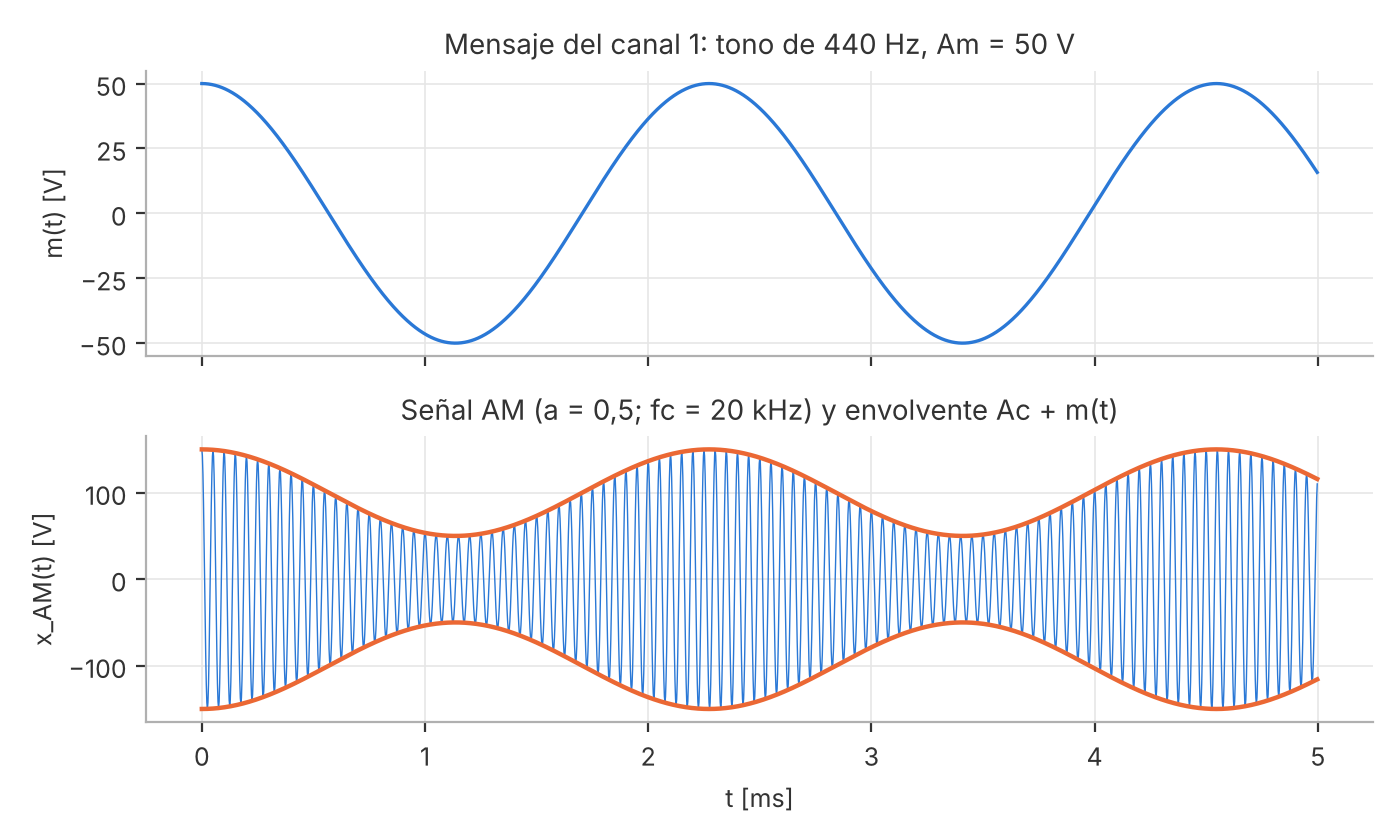
\includegraphics[width=0.85\textwidth]{figs/am_tono_tiempo.png}
  \caption{Tono de 440 Hz y señal AM con $a=0,5$.}
  \label{fig:am_tiempo}
\end{figure}
\begin{figure}[H]
  \centering
  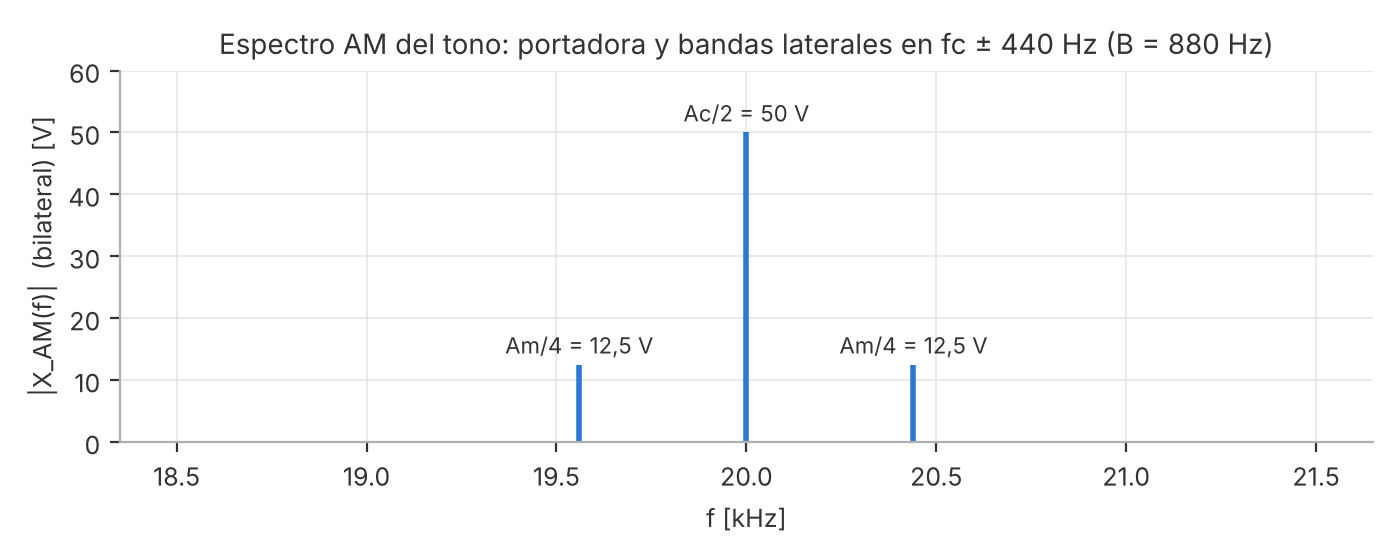
\includegraphics[width=0.85\textwidth]{figs/am_tono_espectro.png}
  \caption{Espectro de líneas de la señal AM del tono.}
  \label{fig:am_espectro}
\end{figure}

Los espectros de FM y PM (Figura \ref{fig:ang_esp}) coinciden con las líneas teóricas $\frac{A_c}{2}\lvert J_n(\beta)\rvert$:
\begin{itemize}
  \item Con $\beta=0,2$ sólo son significativas la portadora y un par de laterales de $5$ V. El ancho de banda es prácticamente el mismo que en AM.
  \item Con $\beta=5$ la portadora casi desaparece ($J_0(5)=-0,178$) y la potencia se reparte entre unas $6$ laterales significativas a cada lado. La banda de Carson de $5280$ Hz contiene el $98\%$ de la potencia, que coincide con el ancho de banda medido con el criterio de potencia significativa.
  \item PM con $\beta=5$ produce el mismo espectro que FM con $\beta=5$.
\end{itemize}

\begin{figure}[H]
  \centering
  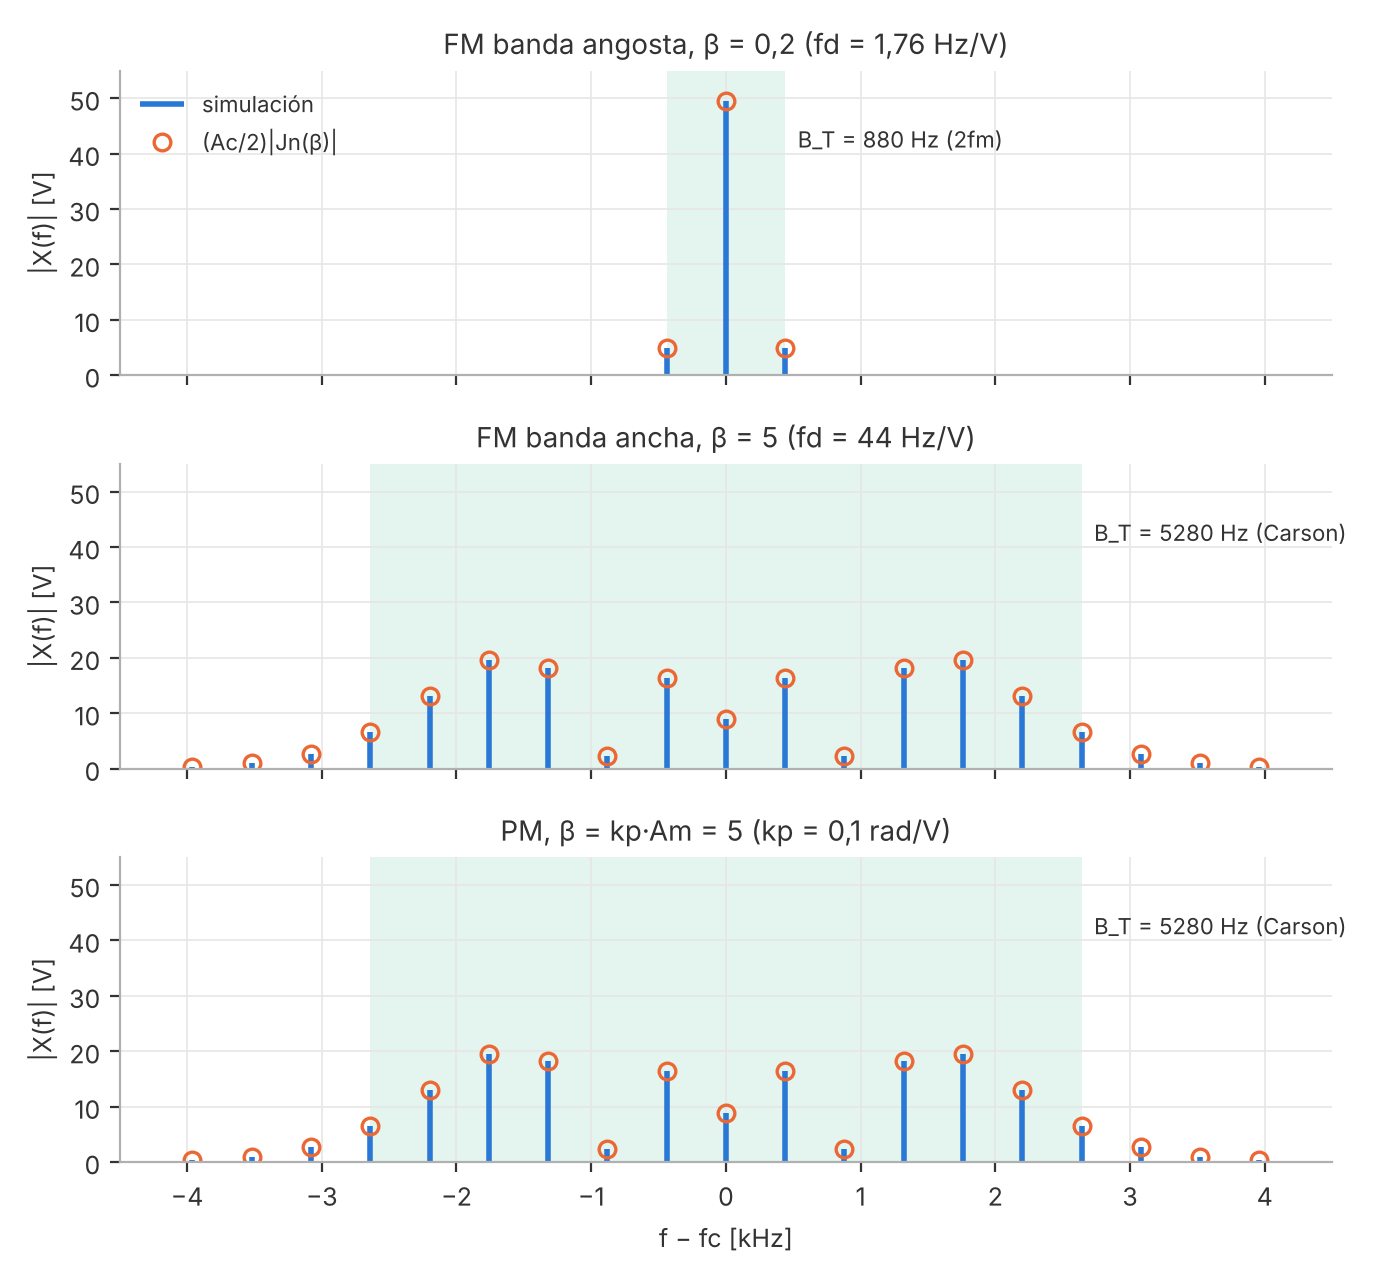
\includegraphics[width=0.85\textwidth]{figs/angular_tono_espectros.png}
  \caption{Espectros de líneas de FM ($\beta=0,2$ y $\beta=5$) y PM ($\beta=5$) frente a las funciones de Bessel.}
  \label{fig:ang_esp}
\end{figure}

\begin{table}[H]
  \centering
  \begin{tabular}{lccccc}
    \toprule
    Esquema & $P_T$ & $P_c$ teórica / simulada & $P_B$ & $E\%$ & $B_T$ \\
    \midrule
    AM, $a=0,5$ & 5625 W & 5000 W / 5000,0 W & 625,0 W & 11,11 \% & 880 Hz \\
    FM, $\beta=0,2$ & 5000 W & 4900,7 W / 4900,7 W & 99,3 W & -- & 1056 Hz \\
    FM, $\beta=5$ & 5000 W & 157,7 W / 157,7 W & 4842,3 W & -- & 5280 Hz \\
    PM, $\beta=5$ & 5000 W & 157,7 W / 157,7 W & 4842,3 W & -- & 5280 Hz \\
    \bottomrule
  \end{tabular}
  \caption{Potencias y ancho de banda del canal 1.}
\end{table}

\begin{table}[H]
  \centering
  \begin{tabular}{lcccc}
    \toprule
    Esquema & $S_i/N_i$ & $S_o/N_o$ (sim. / teo.) & Ganancia (sim. / teo.) & Fidelidad \\
    \midrule
    AM, $a=0,5$ & 38,1 dB & 31,4 / 31,6 dB & 0,215 / 0,222 & 31,4 dB \\
    FM, $\beta=0,2$ & 36,8 dB & 28,3 / 28,4 dB & 0,142 / 0,144 & 28,3 dB \\
    FM, $\beta=5$ & 29,8 dB & 56,1 / 56,3 dB & 434 / 450 & 49,5 dB \\
    PM, $\beta=5$ & 29,8 dB & 51,4 / 51,5 dB & 147 / 150 & 47,9 dB \\
    \bottomrule
  \end{tabular}
  \caption{Relaciones S/N del canal 1 en el sistema FDM ($\eta=10^{-3}$ W/Hz).}
  \label{tab:snr_tono}
\end{table}

Con el tono:
\begin{itemize}
  \item En AM la ganancia de conversión es $2E=0,22$, menor que $1$, como predice el libro. El $88,9\%$ de la potencia transmitida está en la portadora y no aporta información.
  \item FM de banda angosta tiene una ganancia aún menor ($0,14$): ocupa el mismo ancho de banda que AM y no mejora la S/N.
  \item FM de banda ancha ($\beta_m=12$) entrega $56,1$ dB a la salida, $24,7$ dB más que AM, aunque su $S_i/N_i$ es menor (entra más ruido por el filtro de $5280$ Hz). Es el intercambio ancho de banda-relación S/N. En FM y PM de banda ancha la fidelidad ($49,5$ y $47,9$ dB) queda por debajo de $S_o/N_o$: el filtro de Carson descarta el $2\%$ de la potencia de la señal y eso agrega una pequeña distorsión.
  \item PM queda $4,7$ dB por debajo de FM con el mismo $\beta$ y el mismo ancho de banda (teoría: $10\log 3=4,77$ dB).
\end{itemize}

\subsection{Canal 2: La Marcha Imperial}
\begin{figure}[H]
  \centering
  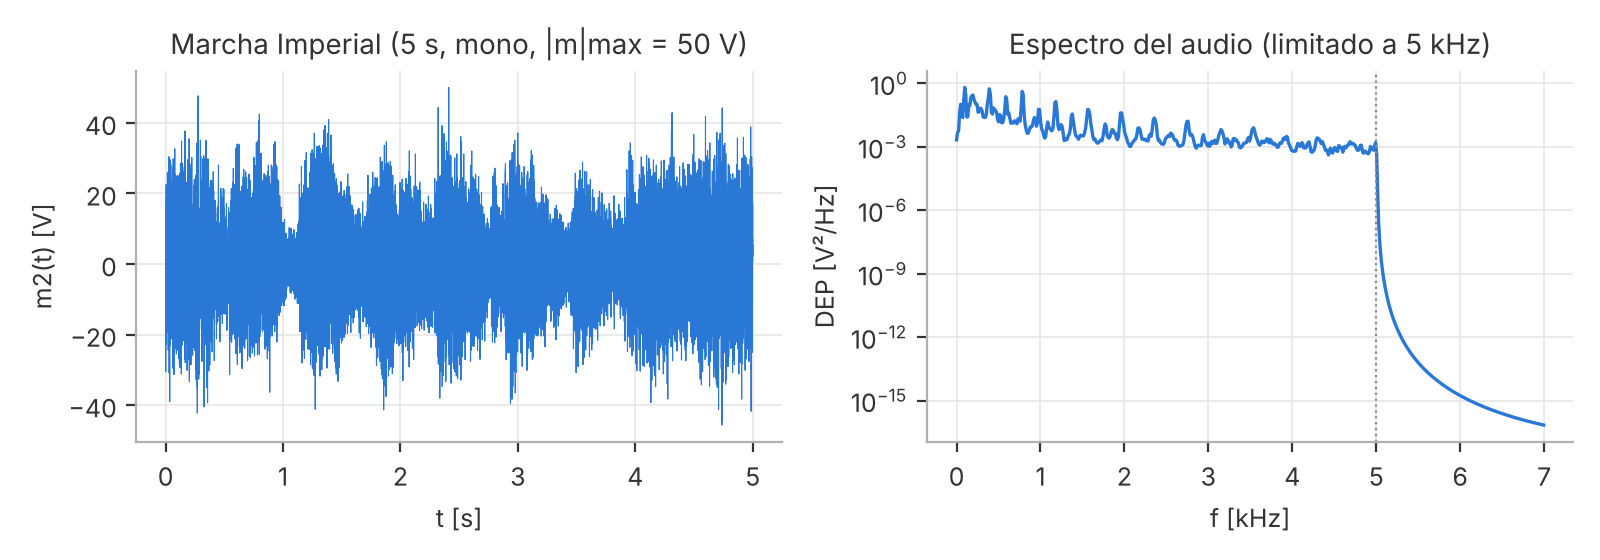
\includegraphics[width=0.95\textwidth]{figs/audio_mensaje.png}
  \caption{Fragmento de audio utilizado como mensaje del canal 2 y su densidad espectral.}
  \label{fig:audio}
\end{figure}

La Figura \ref{fig:fdm} muestra la densidad espectral de la señal multicanal recibida. En AM el canal de audio es una portadora muy intensa con bandas laterales de baja potencia. En FM de banda ancha la potencia se esparce en unos $50$ kHz. En todos los casos la banda de guarda evita el solapamiento: la potencia del canal de audio que se filtra al canal del tono (diafonía) es menor que $4\times 10^{-5}$ W, más de $110$ dB por debajo de la señal.

\begin{figure}[H]
  \centering
  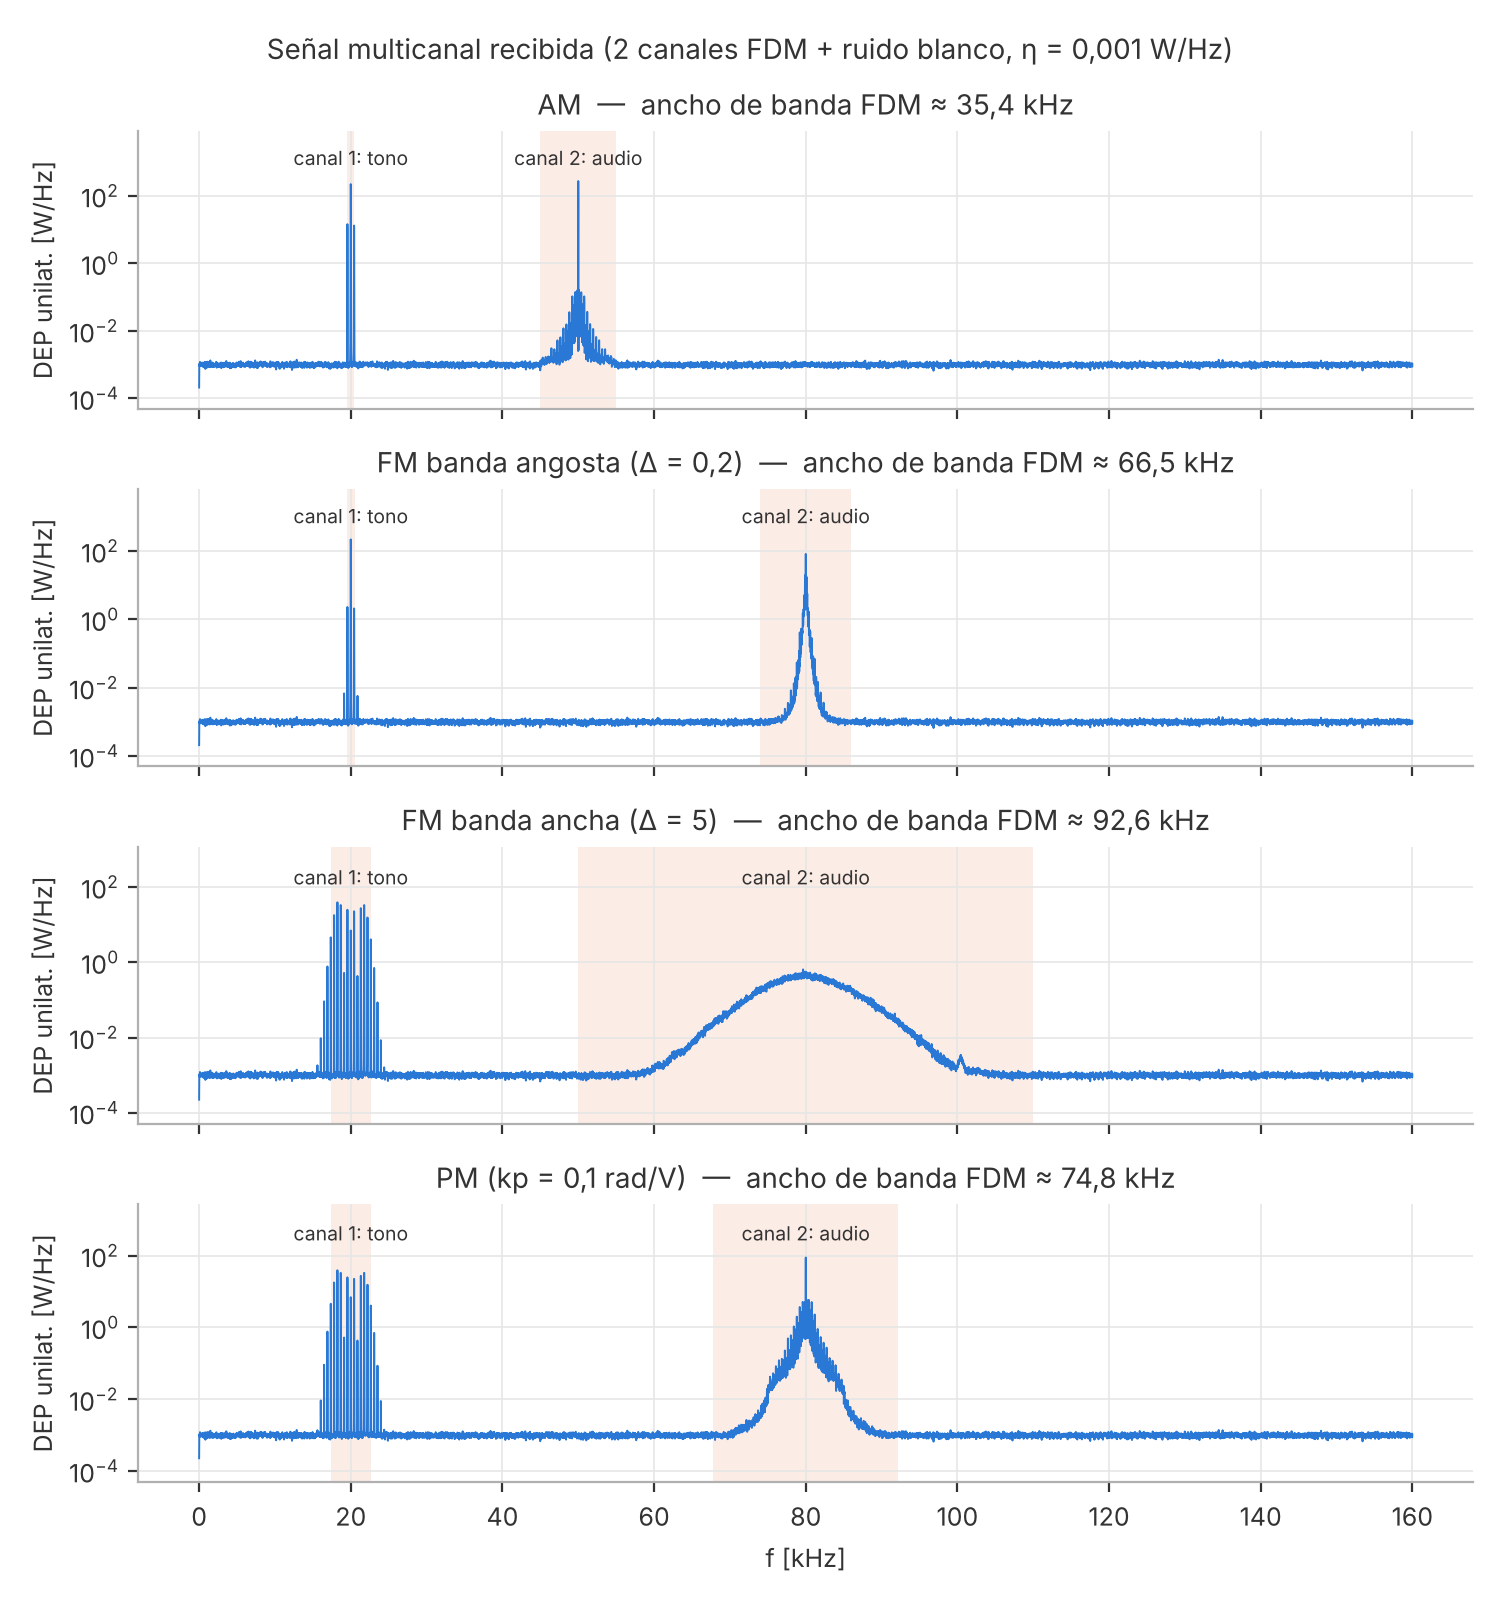
\includegraphics[width=0.95\textwidth]{figs/fdm_espectros.png}
  \caption{Densidad espectral de la señal FDM recibida (tono + audio + ruido) para cada esquema. Las franjas indican la banda de cada filtro de canal.}
  \label{fig:fdm}
\end{figure}

\begin{table}[H]
  \centering
  \small
  \setlength{\tabcolsep}{4pt}
  \begin{tabular}{lcccccc}
    \toprule
    Esquema & $P_T$ & $E\%$ & $B_T$ Carson / 98\% & $S_i/N_i$ & $S_o/N_o$ (sim. / teo.) & Fidelidad \\
    \midrule
    AM & 5050,9 W & 1,01 \% & 10 kHz & 27,1 dB & 10,1 / 10,1 dB & 10,1 dB \\
    FM, $\Delta=0,2$ & 5000 W & -- & 12 kHz / -- & 26,2 dB & 6,6 / 6,9 dB & 6,6 dB \\
    FM, $\Delta=5$ & 5000 W & -- & 60 / 24,8 kHz & 19,2 dB & 34,6 / 34,9 dB & 34,5 dB \\
    PM, $k_p=0,1$ & 5000 W & -- & 24,4 / 7,3 kHz & 23,1 dB & 30,0 / 30,1 dB & 29,9 dB \\
    \bottomrule
  \end{tabular}
  \caption{Canal 2 (audio) en el sistema FDM ($\eta=10^{-3}$ W/Hz).}
  \label{tab:fdm}
\end{table}

\begin{figure}[H]
  \centering
  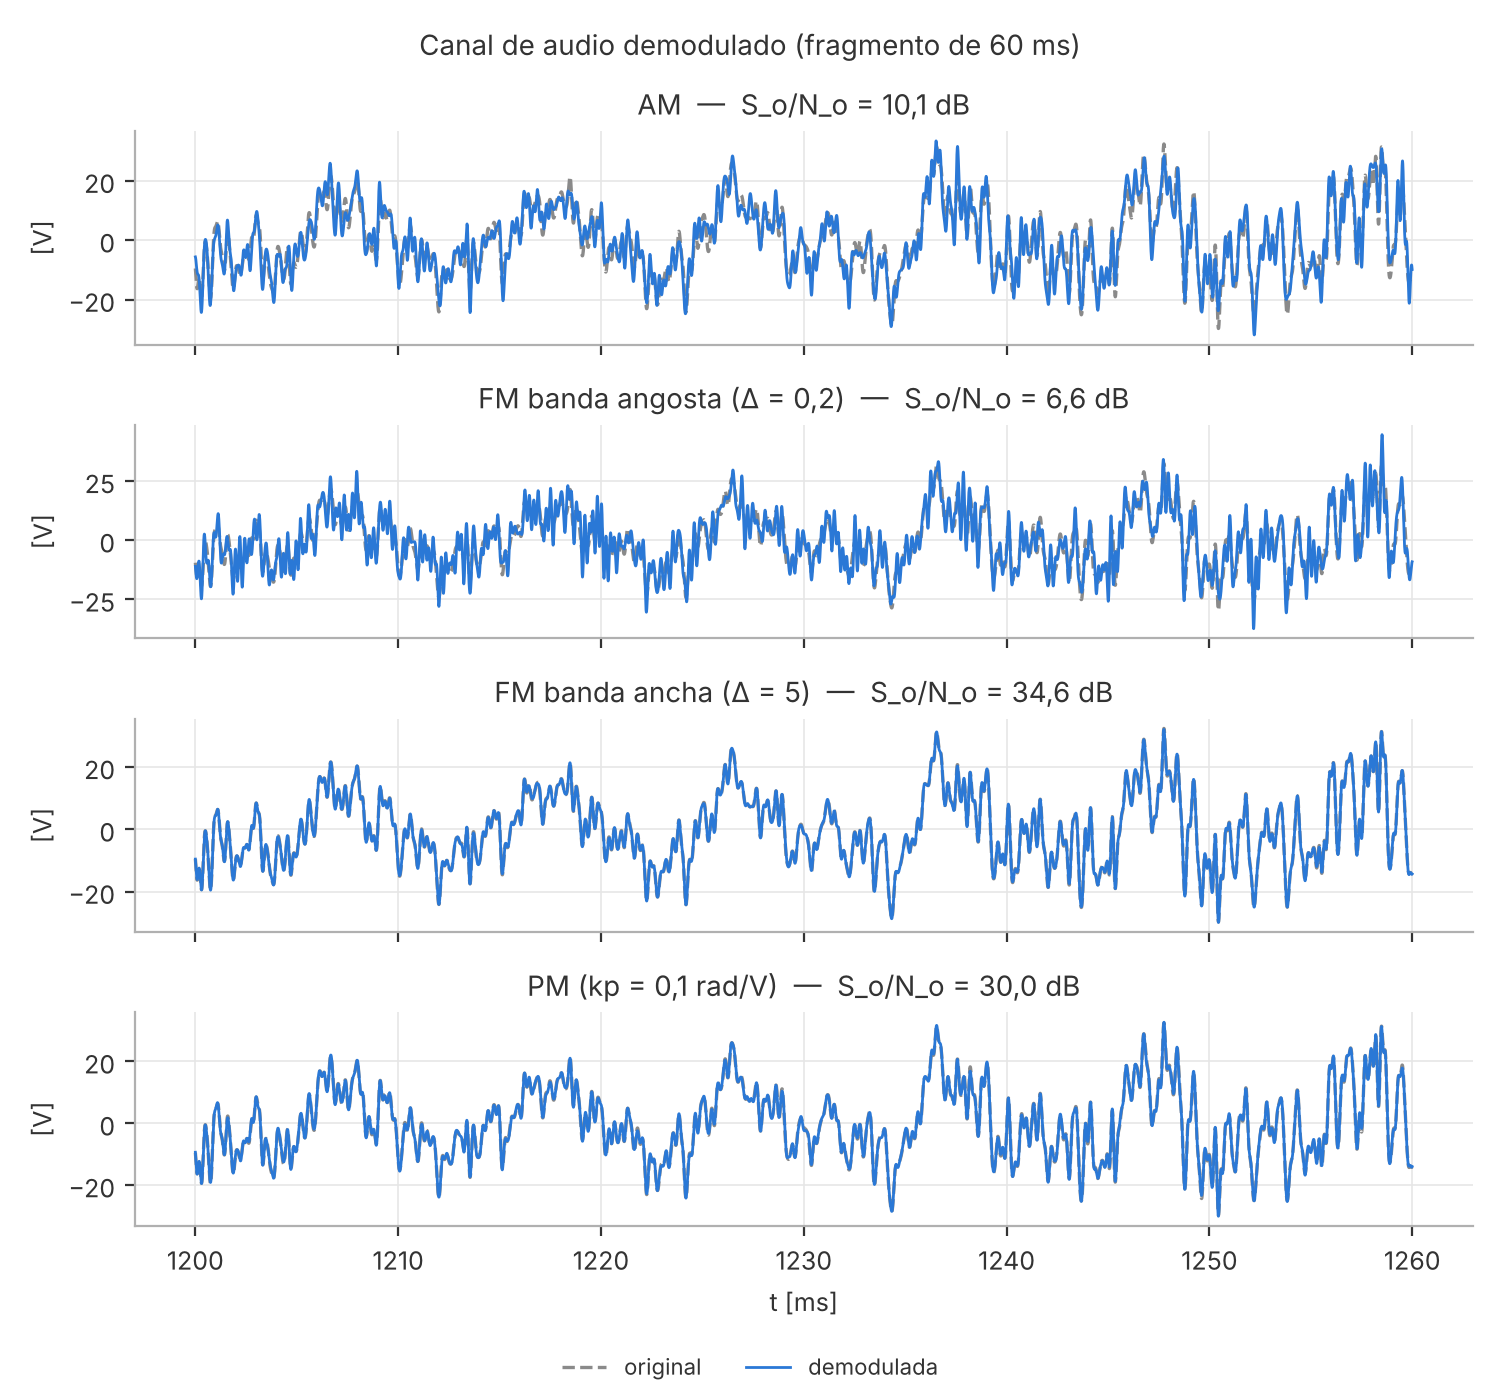
\includegraphics[width=0.9\textwidth]{figs/fdm_audio_demodulado.png}
  \caption{Fragmento de 60 ms del audio original y demodulado con cada esquema.}
  \label{fig:audio_dem}
\end{figure}

Con el audio:
\begin{itemize}
  \item El rendimiento de AM es $1,01\%$, frente al $11,11\%$ del tono con un índice parecido. El audio tiene picos grandes y potencia media baja ($\langle m_n^2\rangle =0,041$ contra $0,5$ del tono), y la portadora se dimensiona para los picos. La ganancia de conversión queda en $2E=0,02$ y la salida tiene un soplido audible ($S_o/N_o=10,1$ dB).
  \item FM de banda angosta da $6,6$ dB: ocupa el mismo ancho de banda que AM sin aprovechar la expansión de banda.
  \item FM de banda ancha entrega $34,6$ dB, $24,5$ dB más que AM con la misma potencia y el mismo ruido, y el audio se escucha prácticamente limpio, a cambio de $6$ veces el ancho de banda.
  \item El $98\%$ de la potencia FM cabe en $24,8$ kHz, menos de la mitad de lo que da Carson ($60$ kHz), porque la desviación máxima sólo se alcanza en los picos del audio. En PM ocurre lo mismo ($7,3$ kHz contra $24,4$ kHz).
  \item PM entrega $30$ dB. Con el mismo $k_p$ que en el canal 1, su ancho de banda ($24,4$ kHz) depende de la pendiente máxima del audio y no de su amplitud, a diferencia de FM.
  \item Todas las mediciones coinciden con las expresiones teóricas con diferencias de $0,3$ dB como máximo. Sin ruido, la fidelidad de todos los esquemas supera los $68$ dB, así que la degradación se debe al ruido del canal y no a los moduladores.
\end{itemize}

\subsection{Señales para Escuchar}
En la carpeta \texttt{assets/audio} se generan los siguientes archivos, que se pueden reproducir desde el cuaderno \texttt{codigo/proyecto2.ipynb}:
\begin{itemize}
  \item \texttt{audio\_original.wav} y \texttt{tono\_original.wav}: los mensajes de cada canal.
  \item \texttt{audio\_am\_demodulado.wav}, \texttt{audio\_fm\_ba\_demodulado.wav},\\ \texttt{audio\_fm\_bw\_demodulado.wav} y \texttt{audio\_pm\_demodulado.wav}: el audio recuperado con cada esquema.
  \item \texttt{tono\_am\_demodulado.wav}, \texttt{tono\_fm\_ba\_demodulado.wav},\\ \texttt{tono\_fm\_bw\_demodulado.wav} y \texttt{tono\_pm\_demodulado.wav}: el tono recuperado con cada esquema.
\end{itemize}

\section{Conclusiones}
\begin{itemize}
  \item \textbf{Eficiencia de potencia.} AM desperdicia la mayor parte de la potencia en la portadora: $88,9\%$ con el tono y $99\%$ con la música. A cambio, el receptor es simple (un detector de envolvente). En FM y PM la potencia es constante ($A_c^2/2$) y el índice sólo la redistribuye entre portadora y laterales. Con $\beta=5$, el $97\%$ va a las bandas laterales, que son las que llevan la información.
  \item \textbf{Eficiencia espectral.} AM y FM de banda angosta ocupan $2f_m$ ($\beta_m=2$) y son las más eficientes en ancho de banda. FM de banda ancha necesitó $5280$ Hz para el tono y $60$ kHz para el audio ($\beta_m=12$), y en el sistema FDM eso llevó el ancho de banda total de $35,4$ kHz (AM) a $92,6$ kHz.
  \item \textbf{Calidad (fidelidad).} Con la misma potencia transmitida y el mismo ruido, FM de banda ancha mejoró la S/N de salida en unos $25$ dB respecto de AM, tanto con el tono como con la música. Las mediciones coincidieron con las expresiones de Briceño.
  \item \textbf{FM banda angosta frente a banda ancha.} La señal demodulada en banda angosta tiene peor S/N que en AM, porque ocupa el mismo ancho de banda y tiene una ganancia de conversión menor. En banda ancha la señal demodulada es mucho más limpia, a costa de más espectro.
  \item \textbf{PM.} Con el tono tiene el mismo espectro que FM del mismo $\beta$, pero $4,7$ dB menos de S/N a la salida. Con el audio, su ancho de banda depende de la pendiente del mensaje.
  \item \textbf{Multicanal.} La multiplexación por división de frecuencia funcionó sin diafonía apreciable al respetar las bandas de guarda. El ancho de banda total del sistema es la suma de los anchos de cada canal más las guardas, así que la elección de la modulación de cada canal determina cuánto espectro necesita el sistema completo.
\end{itemize}
En resumen, AM es barata en ancho de banda y en receptor pero ineficiente en potencia y sensible al ruido. FM de banda ancha intercambia ancho de banda por calidad, y por eso se usa en radiodifusión de alta fidelidad.

\appendix
\section{Anexo: Código}
\begin{itemize}
  \item \texttt{codigo/modulacion.py}: moduladores, demoduladores, canal con ruido, sistema FDM y generación de figuras, audios y \texttt{assets/resultados.json}. Se ejecuta con \texttt{python3 codigo/modulacion.py} desde la raíz del proyecto.
  \item \texttt{codigo/proyecto2.ipynb}: cuaderno que corre la simulación, muestra los gráficos y reproduce los audios.
  \item \texttt{codigo/requirements.txt}: dependencias. Se instalan con:\\
  \hspace*{1em}\texttt{pip install -r codigo/requirements.txt}
\end{itemize}

\end{document}
